% Archivo: capitulos/capitulo2.tex
\chapter{Conceptos Fundamentales}

\section{Objetivos de este capítulo}
En este capítulo, abordaremos los conceptos fundamentales de \textbf{sistema}, \textbf{balance de materia} y \textbf{balance de energía}, aplicándolos al funcionamiento de una central térmica. En lugar de presentar definiciones abstractas desde el inicio, analizaremos cómo estos principios se aplican en la generación de electricidad, para finalmente formalizar los conceptos clave.



\section{Introducción: Central Térmica}
En capítulos previos  \hl{¿CUAL?}, mencionamos que una central térmica es aquella que impulsa la turbina con vapor de agua, el cual se produce gracias al calor generado al quemarse (oxidarse) un combustible fósil como gas, petróleo, carbón.  Veamos entonces las etapas básicas de una central térmica, como se muestra en la Figura \ref{fig:CentralTermica}:

\begin{itemize}
    \item \textbf{Vaporización del agua}: Una corriente de agua se vaporiza gracias al calor producido por la combustión. El agua circula por un conjunto de cañerías que atraviesan una caldera, donde ocurre la combustión.
    
    \item \textbf{Expansión del vapor}: El vapor generado en la caldera (que tiene alta temperatura y presión) se dirige mediante cañerías a la turbina. Allí, el vapor mueve los álabes de este dispositivo, transformando la energía acumulada en el fluido en energía mecánica (de movimiento).
    
    \item \textbf{Condensación del vapor}: El vapor que abandona la turbina (con baja presión y temperatura) se dirige a un intercambiador de calor, donde se condensa por completo al retirarle parte de su energía, mediante una corriente de refrigerante provista por una torre de enfriamiento o tomada de un cauce de agua natural directamente).
    
    \item \textbf{Bombeo del agua}: El agua en estado líquido se bombea a alta presión para reingresar a la caldera, continuando así el ciclo de manera cíclica.
\end{itemize}

El agua que circula a través de los dispositivos (caldera, turbina, condensador y bomba) es la encargada de realizar el transporte de la energía (se lleva la energía de la combustión y la deja en la turbina). En este caso, el agua recibe el nombre de \emph{fluido de trabajo} o \emph{fluido intermediario}

\begin{figure}[htbp]
    \centering
    \includegraphics[scale=0.75]{graphics/centraltermica.jpg}
    \caption{Procesos básicos involucrados en una central térmica.}
    \label{fig:CentralTermica}
\end{figure}



\section{Sistema abierto o volumen de control}

Teniendo en mente el funcionamiento de una central térmica, supongamos que queremos analizar termodinámicamente el agua que circula por una cañería dentro de la caldera. Para ello, tracemos una línea imaginaria que abarque esa cañería, como se muestra en la Figura \ref{fig:EleccionSistema} (recuadro rojo). Esta elección nos permite definir tres regiones:

\begin{figure}[htbp]
    \centering
    \includegraphics[scale=0.75]{graphics/SistemaAbiertoCaldera.jpg}
    \caption{Elección de un sistema.}
    \label{fig:EleccionSistema}
\end{figure}

\begin{itemize}
    \item La región dentro del recuadro, que es el objeto de nuestro análisis y recibirá el nombre de \textbf{sistema}.
    
    \item  La región fuera del recuadro, que interactúa con el sistema que llamaremos \textbf{medio} o \textbf{entorno}
    
    \item La línea que delimita el recuadro, que separa el sistema del medio llamad \textbf{límite o frontera}.
\end{itemize}

Si observamos el recuadro rojo (el límite del sistema), notaremos que hay una corriente de agua que entra y sale de él, lo que significa que la región es atravesada por una cantidad determinada de materia. A este tipo de sistema se lo conoce como \textbf{sistema abierto} o \textbf{volumen de control}. Además, dado que el agua se vaporiza gracias al calor de la combustión, el sistema también intercambia energía con el medio.


Podemos entonces establecer la siguiente definición:



\begin{definicion}{Sistema Abierto}
Un sistema abierto o \textbf{volumen de control} es una región del espacio seleccionada para su análisis, a través de cuya frontera puede existir flujo de masa además de energía.
\end{definicion}

\subsection{Lo que tenés que saber sobre los sistemas abiertos}
Las definiciones académicas son importantes, pero lo esencial es aprender a aplicar estos conceptos en la resolución de problemas. Para ello, tené en cuenta lo siguiente:

\begin{enumerate}
         \item En términos matemáticos, al definir un sistema termodinámico estamos definiendo un sistema de ecuaciones que nos permita (o no) resolver un problema. En otras palabras, si el sistema termodinámico no está bien definido, problablemente tendremos más incógnitas que ecuaciones. 

    \item La selección del sistema es clave en el análisis termodinámico; desarrollar criterio para elegirlo es parte fundamental del aprendizaje.
    \item Inicialmente, este criterio se adquiere mediante prueba y error.
    
    \item La elección del sistema no tiene que coincidir con algo físico: en este caso, elegimos la cañería dentro de la caldera, pero podríamos haber seleccionado toda la caldera, la turbina, el condensador, la bomba o toda la central o la mitad de esta.
   \end{enumerate}   


\subsection{Otros sistemas}
Además de los sistemas abiertos, hay otros dos tipos: el sistema cerrado y el sistema aislado.

El sistema cerrado es aquel a través de cuyos límites hay intercambio de energía, pero no de materia. Es decir, la cantidad de masa en su interior no cambia.

Por su parte, el sistema aislado es aquel en el que no hay intercambios ni de materia ni de energía con el medio. Este sistema, que a simple viste parece inútil desde el punto de vista termodinámico, se emplea para definir el estado de equilibrio de un sistema.
\hl{donde ampliamos esto?}


\section{Balance de materia}

El balance de materia constituye uno de los pilares fundamentales en el estudio de los sistemas termodinámicos y de los procesos de ingeniería química. En términos prácticos, puede interpretarse como un proceso de contabilidad en el que se registran las masas que ingresan a un sistema, las que egresan y la masa que permanece dentro de sus límites. El fundamento de este análisis es el \emph{principio de conservación de la masa}, el cual establece que la materia no se crea ni se destruye, sino que se conserva.

Para aplicar este principio es necesario definir un \emph{volumen de control}, es decir, una región del espacio seleccionada para el análisis. A lo largo de este capítulo se adoptará como volumen de control la cañería por la cual circula el agua en el interior de la caldera. Este enfoque permite analizar el comportamiento del fluido a medida que ingresa al sistema, se calienta y finalmente lo abandona.

\subsection{Estado transitorio: fase de llenado}

Consideremos el caso de una instalación recién construida que se encuentra inicialmente vacía. Al iniciar el proceso de llenado, el fluido comienza a ingresar al volumen de control definido por la cañería del sistema. Durante esta etapa existe una entrada de masa, pero no se observa aún una salida, lo que produce una acumulación progresiva de fluido en el interior de las conducciones.

En estas condiciones, la cantidad de materia contenida dentro del volumen de control varía con el tiempo. Este comportamiento se denomina \emph{estado transitorio} y se caracteriza precisamente por la existencia de acumulación de masa dentro del sistema.

\subsection{Estado estacionario: operación en régimen permanente}

Una vez que la planta alcanza sus condiciones normales de operación y el fluido completa el circuito, el sistema entra en una fase de estabilidad. En este régimen, el volumen de control ya no acumula materia: toda la masa que ingresa por la sección de entrada es simultáneamente desplazada y evacuada por la sección de salida.

Este comportamiento se denomina \emph{estado estacionario} o \emph{régimen permanente} y se caracteriza porque las propiedades macroscópicas del sistema permanecen constantes en el tiempo. En una central térmica, este tipo de operación es el más habitual durante el funcionamiento normal del ciclo. Por ejemplo, el caudal de agua que ingresa a la caldera en estado líquido es igual al caudal de vapor que egresa, despreciando pérdidas menores.

\subsection{Necesidad de una descripción en términos de flujo}

Dado que el agua, en sus diferentes estados de agregación, circula de manera continua dentro del ciclo térmico, resulta poco práctico describir el proceso en términos de cantidades fijas de materia. En su lugar, es más conveniente analizar el sistema en términos de flujos, es decir, considerando cuánta masa atraviesa una determinada sección del sistema por unidad de tiempo.

Esta forma de descripción permite vincular el comportamiento del sistema con variables operativas como el régimen de funcionamiento, la capacidad de los equipos y las condiciones de diseño.

\subsection{Caudal másico}

Para cuantificar el ingreso y egreso de materia a través de las fronteras del volumen de control, se introduce el concepto de \textbf{caudal másico}. El caudal másico representa la cantidad de masa que atraviesa una sección del sistema por unidad de tiempo y se denota como $\dot{m}$.

Desde el punto de vista matemático, el caudal másico se define como la derivada temporal de la masa que atraviesa una sección:

\[
\dot{m} = \frac{dm}{dt}
\]

y se expresa habitualmente en unidades de \(\text{kg/s}\). La notación con un punto sobre la variable \( m \) indica, por lo tanto, una tasa de transferencia de masa.

\subsection{Planteo general del balance de materia}

Una vez definido el volumen de control y el concepto de caudal másico, el balance de materia puede plantearse de manera sistemática. En términos generales, para un sistema abierto, la variación de la masa contenida dentro del volumen de control es consecuencia del ingreso y egreso de materia a través de sus fronteras, así como de posibles procesos de generación o consumo.

De forma esquemática, este balance puede expresarse como:

\begin{center}
\emph{la acumulación de masa dentro del sistema es igual a la masa que entra menos la masa que sale, considerando además posibles términos de generación y consumo.}
\end{center}

En muchos sistemas de ingeniería química, y en particular en aquellos donde no ocurren reacciones químicas, los términos de generación y consumo de masa son nulos.

\subsection{Formalismo matemático del balance de materia}

Sobre la base de los conceptos previamente introducidos, el balance de materia puede expresarse en forma rigurosa mediante una formulación matemática integral. La masa contenida dentro de un volumen de control se define como:

\begin{equation}
m_{vc} = \int_{VC} \rho \, dV
\end{equation}

donde $\rho$ es la densidad del fluido y la integración se realiza sobre todo el volumen de control. La variación temporal de la masa almacenada puede entonces expresarse como:

\begin{equation}
\frac{dm_{vc}}{dt} = \frac{d}{dt} \int_{VC} \rho \, dV
\end{equation}

El intercambio de masa entre el volumen de control y su entorno ocurre a través de sus superficies de entrada y salida. El flujo másico a través de una superficie diferencial $dA$ puede expresarse como:

\begin{equation}
\delta \dot{m} = \rho \, \vec{v} \cdot \vec{n} \, dA
\end{equation}

donde $\vec{v}$ es el vector velocidad del fluido y $\vec{n}$ es el vector normal a la superficie. Integrando sobre toda la superficie de control, se obtiene el flujo másico total:

\begin{equation}
\dot{m} = \int_{SC} \rho \, \vec{v} \cdot \vec{n} \, dA
\end{equation}

En muchos problemas de ingeniería, el flujo puede considerarse aproximadamente unidimensional y uniforme sobre una sección transversal. En ese caso, la expresión anterior se simplifica y el caudal másico puede escribirse como:

\begin{equation}
\dot{m} = \rho \, A \, v
\end{equation}

El balance de materia para un sistema abierto puede entonces expresarse como:

\begin{equation}
\text{acumulación} = \text{entrada} - \text{salida} + \text{generación} - \text{consumo}
\end{equation}

En ausencia de reacciones químicas, esta expresión se reduce a:

\begin{equation}
\frac{dm_{vc}}{dt} = \sum_e \dot{m}_e - \sum_s \dot{m}_s
\end{equation}

Esta ecuación es válida tanto para estados transitorios como para estados estacionarios. En particular:

\begin{itemize}
\item En \textbf{estado transitorio}, el término de acumulación es distinto de cero y la masa contenida en el volumen de control varía con el tiempo.
\item En \textbf{estado estacionario}, el término de acumulación se anula y el balance se simplifica a:
\end{itemize}

\begin{equation}
\label{ec:BalanceMateriaEstacionario}
\sum_e \dot{m}_e = \sum_s \dot{m}_s
\end{equation}

Esta expresión indica que, en régimen permanente, la cantidad de masa que entra al sistema es igual a la que sale.




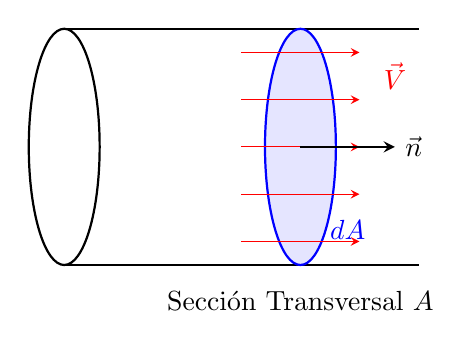
\begin{tikzpicture}[scale=1.5]
    % Dibujo de la tubería (cilindro)
    \draw[thick] (0,1) -- (3,1);
    \draw[thick] (0,-1) -- (3,-1);
    \draw[thick] (0,0) ellipse (0.3cm and 1cm);
    
    % Sección de control dA
    \filldraw[blue!20, opacity=0.5] (2,0) ellipse (0.3cm and 1cm);
    \draw[blue, thick] (2,0) ellipse (0.3cm and 1cm);
    
    % Perfil de velocidades (Flechas)
    \foreach \y in {-0.8,-0.4,0,0.4,0.8} {
        \draw[-stealth, red] (1.5,\y) -- (2.5,\y);
    }
    \node[red] at (2.8,0.6) {$\vec{V}$};
    
    % Vector normal y diferencial de área
    \draw[-stealth, black, thick] (2,0) -- (2.8,0) node[right] {$\vec{n}$};
    \node at (2, -1.3) {Sección Transversal $A$};
    
    % Etiquetas
    \node[blue] at (2.4, -0.7) {$dA$};
\end{tikzpicture}

\section{Balances de energía}
\subsection{El Primer Principio}
No tengo ninguna duda de que, palabras más, palabras menos, aprendiste en asignaturas previas (o incluso en la escuela secundaria) que la energía no se crea ni se destruye, sino que se transforma. En otras palabras, ya tenés bien claro que la energía se conserva. Lo que quizás no tengas tan claro es que esto no es ni más ni menos que el \textbf{Primer Principio de la Termodinámica}, y lo emplearemos como uno de los instrumentos de análisis. Antes de seguir, algunas aclaraciones que considero necesarias sobre principios, leyes y teorías.

\subsubsection{Sobre leyes, principios y teorías}
En el contexto de la ciencia, una ley (o principio) \textbf{describe cierto fenómeno natural por medio de la relación de algunas variables}. Una ley no se demuestra, porque su función es simplemente describir un comportamiento observado en la naturaleza. Sin embargo, una teoría es un conjunto de ideas o suposiciones comprobadas que \textbf{explican} por qué ocurre ese fenómeno.

Para entender mejor esta diferencia, veamos un ejemplo cotidiano:

\begin{itemize}
    \item \textbf{Ley}: Imagina que observas que cada vez que sueltas un objeto, este cae al suelo. Podrías formular una ley que diga: "Todos los objetos cerca de la superficie de la Tierra caen con una aceleración constante de \(9.8 \, \text{m/s}^2\)". Esta ley describe lo que ocurre, pero no explica por qué sucede.
    \item \textbf{Teoría}: Ahora, para explicar por qué los objetos caen, necesitas una teoría. La Teoría de la Gravitación de Einstein (Relatividad General) explica que los objetos caen porque la masa de la Tierra curva el espacio-tiempo a su alrededor, y los objetos simplemente siguen esa curvatura. Esta teoría no se deduce de la ley, sino que se construye a partir de observaciones, experimentos y datos que validan su explicación.
\end{itemize}

En este ejemplo, la ley describe el comportamiento (los objetos caen), mientras que la teoría explica la causa (la curvatura del espacio-tiempo). Es importante destacar que una teoría no se convierte en ley, ni una ley se deduce de una teoría. Ambas son herramientas complementarias: la ley describe, y la teoría explica.

Volviendo al caso de Newton: él formuló la Ley de Gravitación Universal, que describe cómo dos cuerpos se atraen en función de sus masas y la distancia que los separa. Sin embargo, la explicación de por qué ocurre esta atracción no estaba en su ley, sino que llegó más tarde con la Teoría General de la Relatividad de Einstein.

Retomando con nuestra querida Termodinámica: está estructurada sobre cuatro leyes o principios que describen distintos comportamientos de la energía, los cuales iremos viendo conforme avancemos en este libro.


\subsection{La ecuación del Primer Principio para sistemas abiertos}
En el balance de energía aplicaremos el Primer Principio y su ecuación para sistemas abiertos. Esta tiene la siguiente forma:

\begin{equation}
\dot{Q} - \dot{W} + \sum_e \dot{m}_e \left(h + e_c + e_p \right)_e = \sum_s \dot{m}_s\left(h + e_c + e_p\right)_s 
\end{equation}

Vamos a desmenuzar la ecuación: primero diremos que, obviamente, todos los términos representan diferentes tipos de energía.

Los términos $\dot{Q}$ y $\dot{W}$ representan calor y trabajo respectivamente: son las dos maneras en que un sistema intercambia energía con el entorno. Discutiremos esto más adelante. El punto sobre la letra indica que es calor por unidad de tiempo.

\subsection{Ejemplo: Balance de materia y energía en la Central Térmica Güemes}
La Central Térmica Güemes, ubicada en Salta, Argentina, opera con un ciclo Rankine. Supongamos que analizamos el flujo de agua en la caldera:

\begin{itemize}
\item Flujo de entrada de agua líquida: $\dot{m}_e = 600\,\text{kg/s}$
\item Flujo de salida de vapor de agua: $\dot{m}_s = 600\,\text{kg/s}$
\item Entalpía del agua líquida: $h_e = 800\,\text{kJ/kg}$
\item Entalpía del vapor de salida: $h_s = 2800\,\text{kJ/kg}$
\end{itemize}

Dado que no hay acumulación de materia en estado estacionario:

\begin{equation}
600\,\text{kg/s} = 600\,\text{kg/s}
\end{equation}

Para el balance de energía:

\begin{equation}
\dot{Q} = \dot{m} (h_s - h_e) = 600 (2800 - 800) = 1200000\,\text{kW}
\end{equation}

Esto confirma que la energía térmica suministrada permite la transformación de agua en vapor dentro de la caldera.







